\documentclass[a4paper,12pt,twocolumn]{article}
\usepackage[utf8]{inputenc}
\usepackage{graphicx}
\usepackage{natbib}     % omit 'round' option if you prefer square brackets
\usepackage{hyperref}

\title{CM30229 - ICCS}
\author{Adam Jaamour & Tom Slattery}
\date{28th February 2019}

\begin{document}
\maketitle
\thispagestyle{empty}
\clearpage
\setcounter{page}{1}

% ----------------------------------------------------------------------------

\section{Introduction}

Todo:
\begin{itemize}
    \item state goal of research
    \item LEGO Mindstorm EV3 kit
    \item state the different types of sensors used, design reasons (positioning of the sensors for better/optimal readings)
    \item include picture of the robot?
    \item specify approaches using references
    \begin{itemize}
        \item reactive approach using subsumption architecture (Wooldridge, 2009)
        \item --> to allow rover to determine its current situation
        \item using subsumption based on (Brooks, 1991) thesis
    \end{itemize}
\end{itemize}

% ----------------------------------------------------------------------------

\section{Approach}

Todo:
\begin{itemize}
    \item initial design of rover is usually a simple reflex agent (Russell et al., 1995), allows rover to react to state CRASH but no context for recovery is provided
    \item final design: model-based reflex agent (Russell et al., 1995) allows sensors to modify state
    \item explain how sensor reading quality is improved: take multiple readings at once, if readings are outside the bounds of standard deviation from mean, then not considered. Then the remaining readings are averaged to get final reading that the sensors will act on.
    \item include a perception architecture figure?
    \item explain the decision loops and how they affect/set states (describe the states)
    \item describe rover rates of measurements per second
    \item end by formulating hypothesis e.g. "the rover will perform better if threshold is higher, or if measurements per second is higher, or if 
    \item describe the experiment procedure and conditions (e.g. if robot is stuck then restart experiment)
    \item figure showing layout of the track/obstacles?
    \item mention who did what in the rover's design
    \item mention how morphology helps (wings can help it turn in corners)
    \item motor overcompensating
\end{itemize}

\begin{figure*}[ht]
\centering
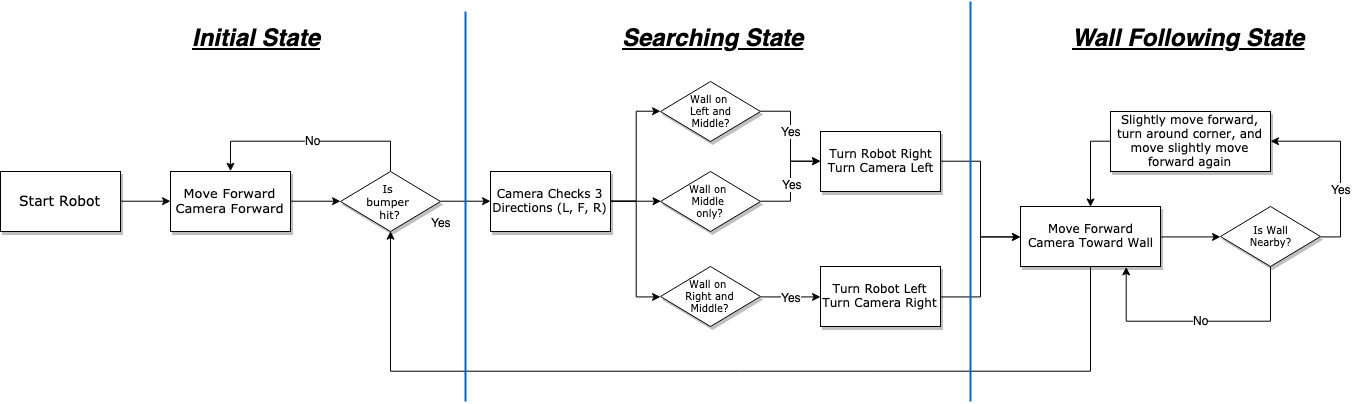
\includegraphics[width=\linewidth]{figures/System-Flowchart.png}
\caption{Flowchart}
  \label{fig:flowchart}
\end{figure*}

% ----------------------------------------------------------------------------

\section{Results}

Todo:
\begin{itemize}
    \item state that results are in line with the hypothesis
    \item place results in table
    \item provide link to youtube video
\end{itemize}

% ----------------------------------------------------------------------------

\section{Discussion}

Todo:
\begin{itemize}
    \item suggest improvements (better quality sensors with less noise? more sensors?)
    \item make arena as consistent as possible (obstacles, wall placement, lighting)
\end{itemize}

% ----------------------------------------------------------------------------

\section{Conclusion}

Todo:
\begin{itemize}
    \item single paragraph
    \item what this research set out to do and the results of the research
\end{itemize}

\bibliographystyle{acm}
\bibliography{bibliography.tex}

\end{document}